\subsection{Implémentation de la caméra}

Le contrôle de la caméra dans notre jeu repose sur un système d’interactions combinées entre le clavier et la souris. Afin de centraliser la logique, nous n’utilisons qu’un seul objet caméra, dont le comportement varie légèrement en fonction du mode de jeu actif. Un paramètre dédié permet de définir le \textit{mode de caméra} courant, influençant certaines actions ou limites de mouvement. Nous distinguons actuellement trois modes principaux :

\url{https://www.youtube.com/watch?v=Lqe8gNZgmzo}

\begin{itemize}
    \item \textbf{Mode Seigneur} : la caméra adopte une vue en 3/4 légèrement inclinée et ne peut pas zoomer au-delà d’une certaine valeur minimale, assurant une vue stratégique du royaume.
    
    \item \textbf{Mode Carte-Monde} : la caméra est orientée plus verticalement, comme une carte vue de dessus. Le zoom est limité vers le haut afin de conserver une vision globale et simplifiée du monde. Ce mode est conçu pour la navigation macro entre les différents royaumes ou zones.

    \item \textbf{Mode Péon} similaire au mode Seigneur dans sa présentation, il ajoute cependant un suivi automatique du personnage contrôlé par le joueur. Contrairement au mode Seigneur, ce mode repose sur l’existence d’un avatar jouable.
\end{itemize}

\begin{figure}[!h]
    \centering
    \begin{subfigure}{0.39\linewidth}
        \centering
        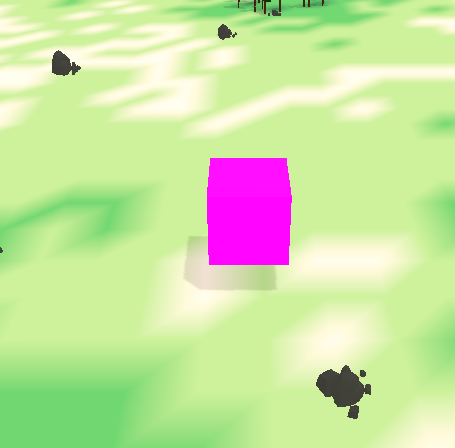
\includegraphics[width=\linewidth]{images/camera_peon.png}
        \caption{Camera mode péon (le cube représente un personnage)}
        \label{fig:image_avant_expansion}
    \end{subfigure}
    \hfill
    \begin{subfigure}{0.4\linewidth}
        \centering
        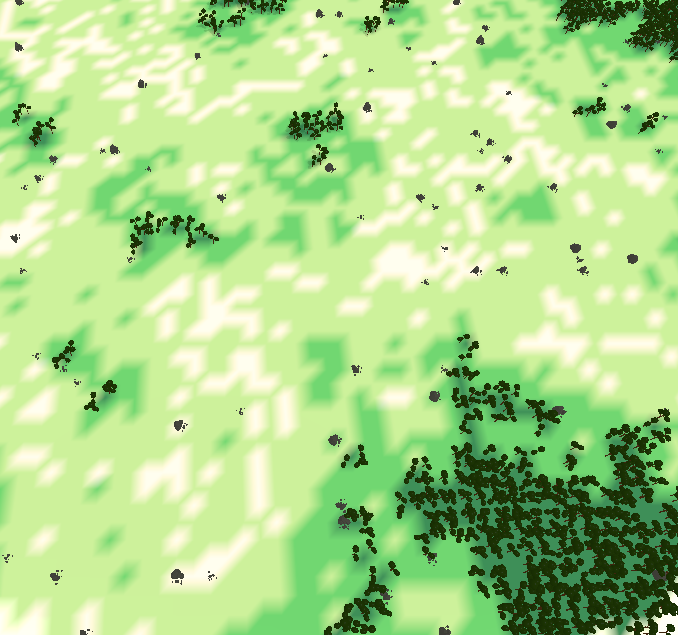
\includegraphics[width=\linewidth]{images/camera_seigneur.png}
        \caption{Camera mode Carte-Monde }
        \label{fig:histo_avant_expansion}
    \end{subfigure}
    \caption{}
\end{figure}

Le déplacement latéral de la caméra est déclenché par la position de la souris : lorsqu’elle s’approche des bords de l’écran, la caméra se déplace dans la direction correspondante. La vitesse de déplacement est proportionnelle à la proximité du curseur avec le bord, rendant le contrôle plus intuitif.
\\ \\
La recentration de la caméra est possible à tout moment via les touches \texttt{Espace} ou \texttt{C}. La cible de recentrage dépend du mode : il s'agit de la position du personnage joueur en mode Péon, ou d’un point arbitraire prédéfini en mode seigneur.
\\ \\
Le zoom est géré via la molette de la souris, modifiant uniquement l'altitude de la caméra. Cette variation de hauteur déclenche également un \textbf{changement automatique de mode} lorsque certaines valeurs seuils sont franchies. Par exemple, un dézoom important bascule la caméra en mode Carte-Monde, tandis qu’un zoom vers l’avant permet de revenir au mode Seigneur ou Péon. Ce système de transition continue renforce la fluidité de la navigation et justifie l'utilisation d’une unique caméra partagée entre les modes.
\\ \\
Afin de garantir une transition naturelle entre les modes, nous avons mis en place une \textbf{zone de seuil élargie} : la caméra entre en mode Carte-Monde uniquement après avoir dépassé une limite haute, et ne revient au mode précédent qu’après avoir atteint une limite basse, évitant ainsi les basculements trop fréquents ou brusques.
\\ \\
Les paramètres relatifs au comportement de la caméra, comme la vitesse de déplacement, les seuils de zoom, ou encore les marges de détection des bords d’écran, sont définis sous forme de constantes, ce qui permet de les ajuster facilement sans avoir à modifier la logique du code.
\\ \\
Enfin, un problème rencontré concernait le comportement de la souris en dehors du canvas du jeu. Lorsque l’utilisateur navigue sur d’autres onglets ou déplace le curseur hors de la fenêtre, la caméra pouvait continuer à se déplacer involontairement. Nous avons donc ajouté une détection explicite de sortie de l’écran, désactivant temporairement le contrôle de la souris jusqu’à son retour dans l’aire de jeu.
\\ \\
En conclusion, nous avons conçu une caméra simple mais polyvalente, capable de s’adapter aux différents contextes de jeu tout en assurant une expérience utilisateur fluide et agréable. Ce système unifié facilite aussi les transitions visuelles et renforce la cohérence entre les différentes phases de gameplay.





